
\documentclass[12pt,a4paper,landscape]{article}
\usepackage[latin1]{inputenc}
\usepackage{amsmath}
\usepackage{amsfonts}
\usepackage{amssymb}
\usepackage{graphicx}
\usepackage{lscape}
\usepackage{multicol}
\usepackage{setspace}
\usepackage[margin=2.5cm]{geometry}
\newcommand{\est}[2]{\begin{array}[t]{c}
\hspace{-.125in}#1\hspace{-.125in}\vspace{-.13in}\\ 
\hspace{-.125in}#2\hspace{-.125in}
\end{array}}
\linespread{1.6}
\newcommand{\arf}{ \underset{f = \mathsf{ 2}}{(1 - \mathsf{  0.00} B+ \est{\mathsf{  0.00}}{(\mathsf{  0.00})}B^\mathsf{2})}}
\newcommand{\nrdiff}{\nabla} 
\newcommand{\nadiff}{\nabla_{\mathsf{12}}}
\newcommand{\ifadf}{ }
\begin{document}
\begin{flushleft}
\thispagestyle{empty}
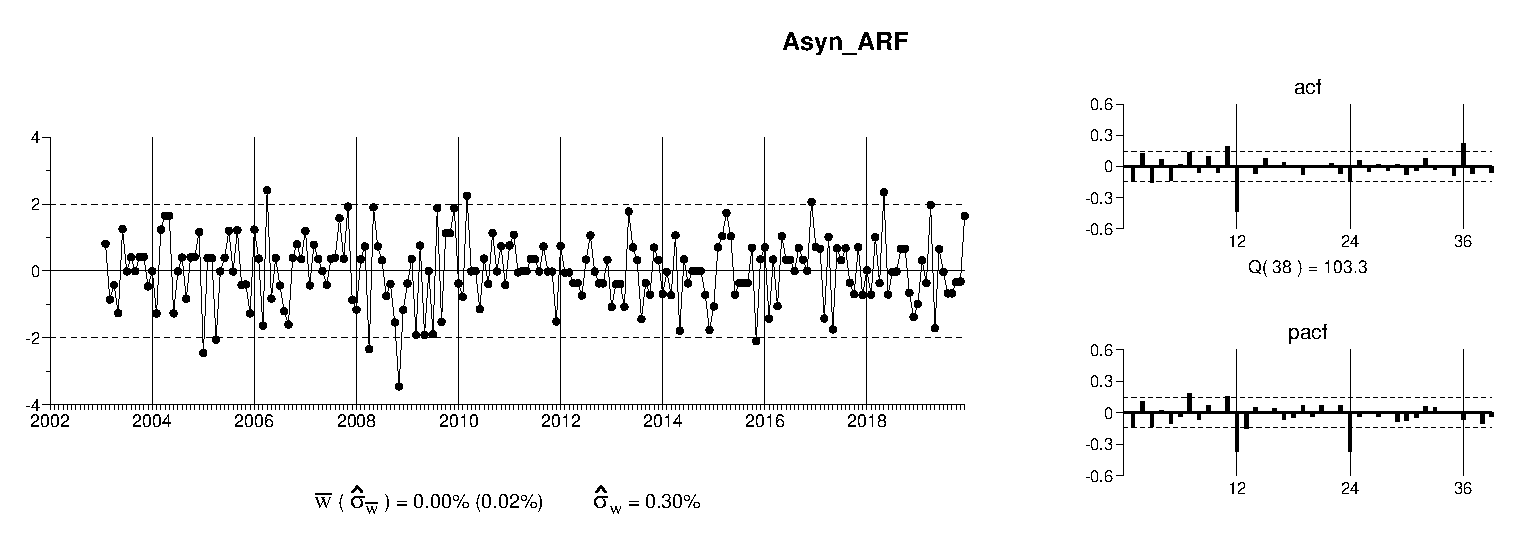
\includegraphics[scale=1]{Asyn_ARF.eps}
\begin{footnotesize}
 $ \arf 
\nrdiff 
\nadiff 
\ifadf \ln \mathsf{IPCM}_{t} = \mathsf{Asyn_ARF_{t}} ; \quad 
\hat{\sigma}_{\mathsf{Asyn_ARF}}=  \mathsf{ 0.30 } \%  $ 

\bigskip 
\begin{multicols}{2}{ 
\begin{tabular}{ccc}
\hline  Obs.  &  Date &  Std. Val. \\ 
\hline 
                       70 &       11/2008 &         -3.45 \vspace{-.12in} \\  
 \end{tabular} 
\\ 
 \columnbreak 
 \singlespacing 
 \underline{\textbf{Comments:}} \\ 
 \bigskip       

% \underline{Action:} 
 } 
\end{multicols} 

\end{footnotesize}
\end{flushleft}
\end{document}
